\documentclass{article}
\usepackage{url}
% \usepackage{showframe}
\usepackage{mathtools}
\usepackage{multirow}
\begin{document}
\title{Ripple Protocol Consensus Algorithm Review}
\author{Peter Todd}
\date{May 11th 2015}
\maketitle

\section{Activities Performed}

Four major activities were performed during the review:

\begin{enumerate}

    \item Reviewed white papers and development documentation at \url{https://ripple.com}.

    \item Reviewed existing third-party criticism.

    \item Setup and run a full node.

    \item Reviewed C++ implementation, specifically the 0.27.4 tag of
        \texttt{rippled}.\footnote{git commit
    \texttt{92812fe7239ffa3ba91649b2ece1e892b866ec2a} from \url{https://github.com/ripple/rippled}}

\end{enumerate}


\section{Overall Architecture}

Ripple has diverged significantly from the original
concept\cite{btcmag-introducing-ripple} of a decentralized network recording
the transferral of money explicitly as debt relationships between parties.
(Figure \ref{fig:orig-ripple}, showing entities A, B, and C participating in a
transaction) While the concept of a debt relationship still exists in the form
of trustlines between participants, the bulk of the codebase and developer
documentation now focuses\footnote{For instance the ``Tutorials'' section of
the Ripple website only explains how to create transactions that modify the
ledger; there is almost no information available on how to actually use the
trustlines feature.} on the use and maintenance of a global ledger of
transactions and account balances.  Additionally a native currency, XRP, has
been added, which is used for anti-spam transaction fees\footnote{A small
amount of XRP is irrevocably destroyed for every transaction.} and to
serve as a universal currency. (Figure \ref{fig:ripple-labs-ripple})

\begin{figure}
    \centering
    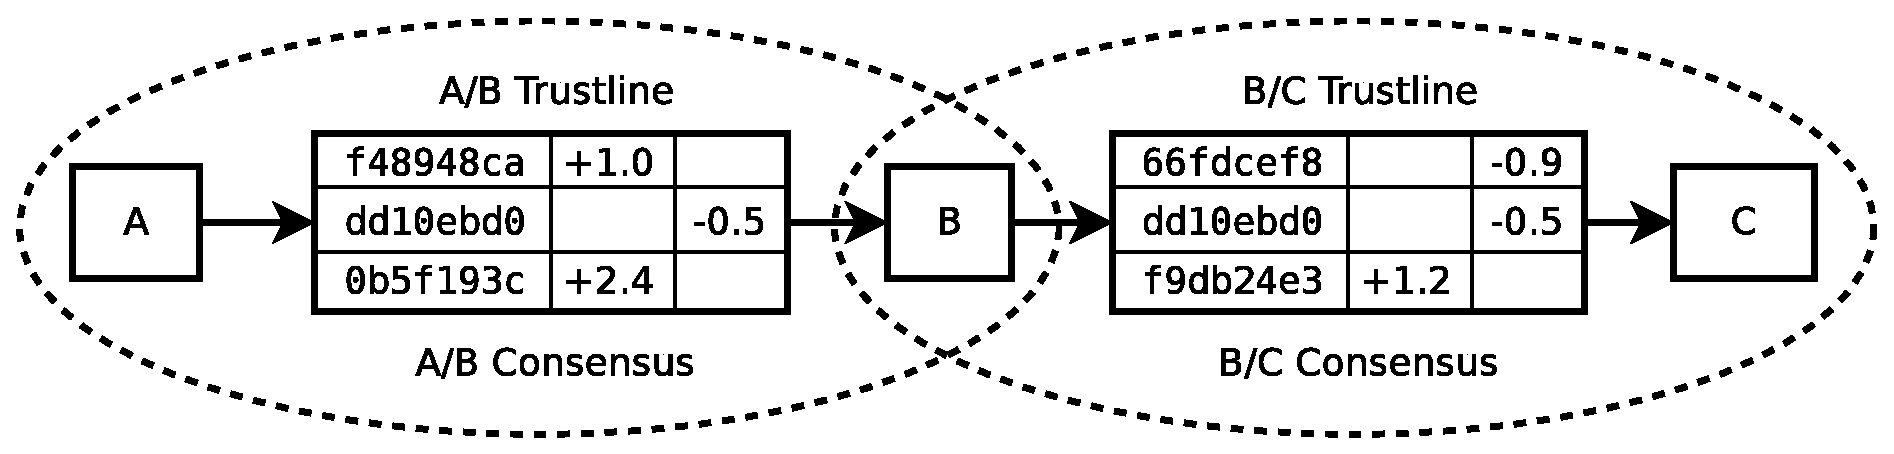
\includegraphics[scale=0.3]{figures/orig-ripple.eps}
    \caption{Original Ripple Architecture}
    \label{fig:orig-ripple}
\end{figure}

\begin{figure}
    \centering
    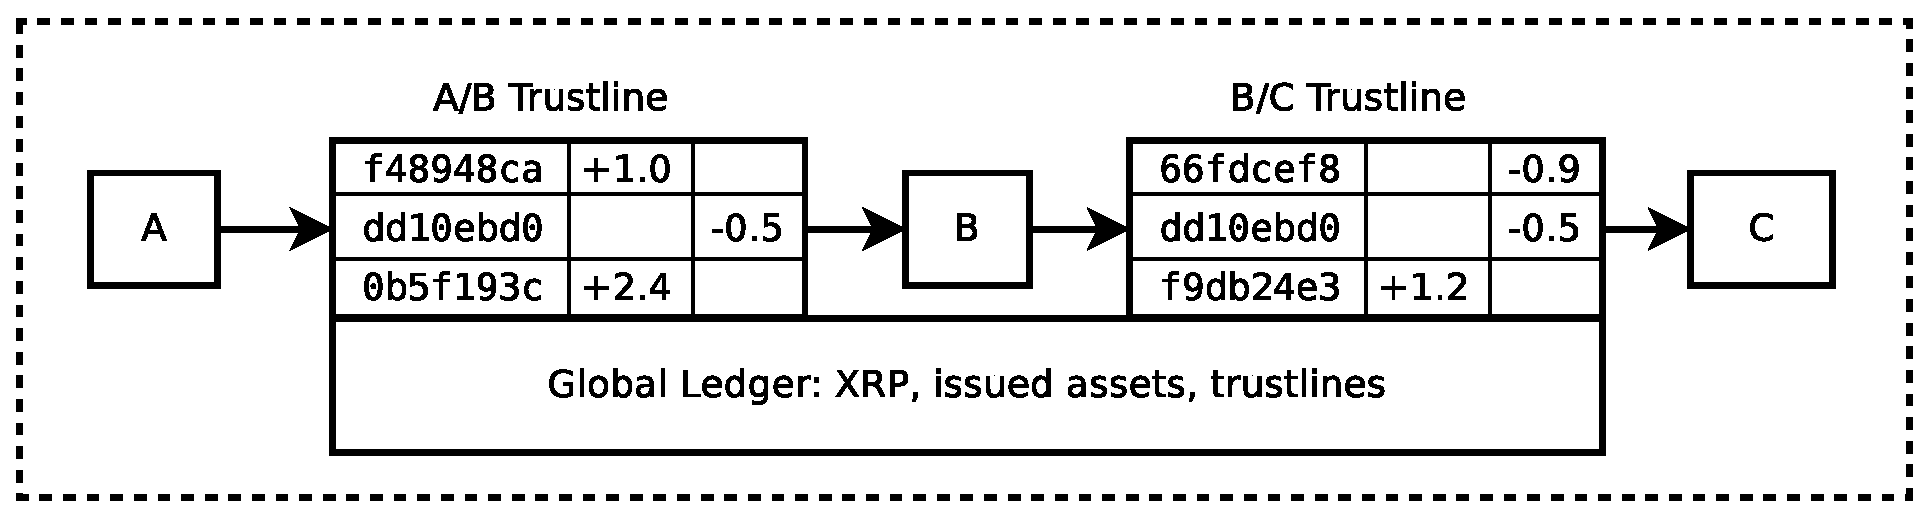
\includegraphics[scale=0.3]{figures/ripple-labs-ripple.eps}
    \caption{Ripple Labs Architecture}
    \label{fig:ripple-labs-ripple}
\end{figure}


\section{Global Ledger}

Figure \ref{fig:ledger-blockchain} shows the basic cryptographic structure of
the Ripple ledger. As with Bitcoin, it consists of a set of chain of blocks,
each consisting of a block header that commits to a previous block and a set of
new transactions for that block. (via a merkle tree) Additionally each block
header also commits to a merkelized trie\footnote{Oddly the trie is not binary,
trading off performance for significantly larger proofs.} of the state of all
account balances. The block chain doesn't itself deal directly with the
consensus protocol. Rather validators sign messages as part of the consensus
protocol, and knowledge of those messages lets Ripple nodes determine the
correct chain.

Developer documentation about exactly how the ledger is structured is somewhat
spotty; the descriptions here are mostly based on direct analysis of the
\texttt{rippled} source code.

\begin{figure}
    \centering
    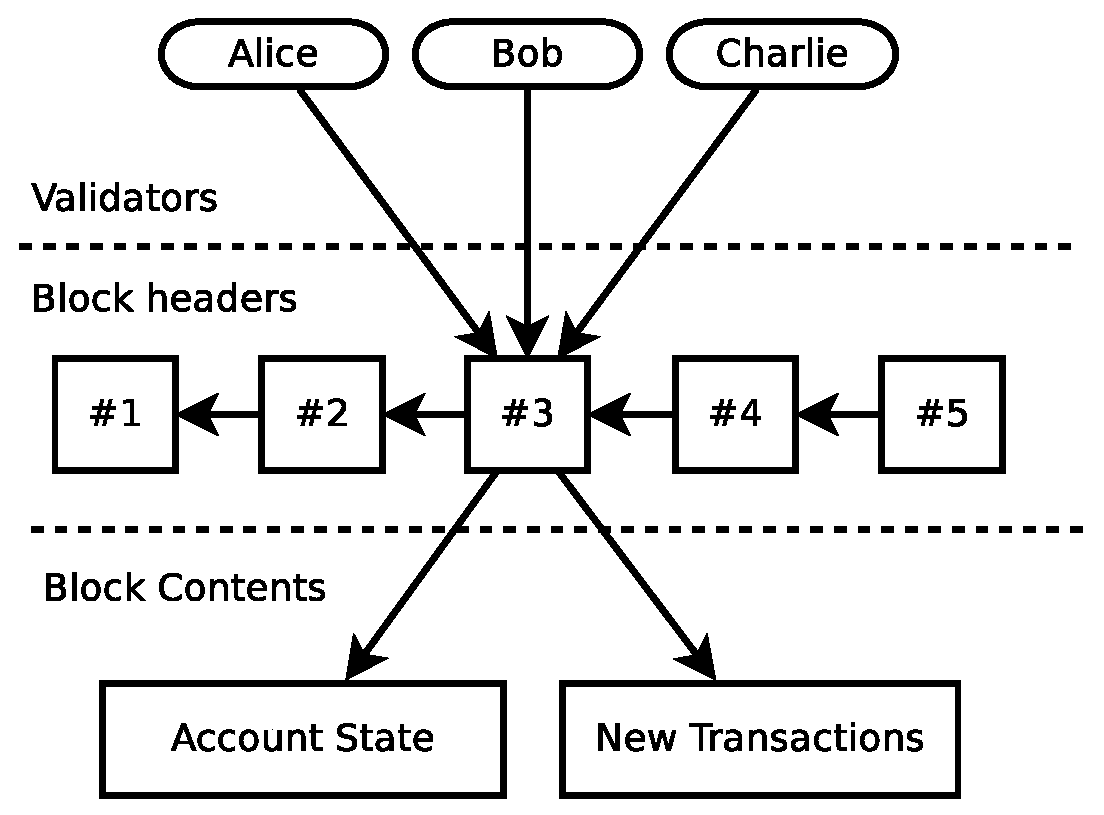
\includegraphics[scale=0.3]{figures/ledger-blockchain.eps}
    \caption{Ripple Ledger Structure}
    \label{fig:ledger-blockchain}
\end{figure}


\subsection{Transactions}

Unlike Bitcoin, transactions increment and decrement account balances; they do
not directly consume the output of other transactions. Transactions are also
used to setup and modify trustlines. To prevent replay attacks, accounts and
transactions have sequence numbers; a transaction is only valid if the Sequence
number is exactly one greater than the last-valided transaction from the same
account. Additionally an optional AccountTxnID field is available for use
within transactions; the transaction is only valid if the sending account's
previously-sent transaction matches the provided hash.

Authentication is performed with a simple signature scheme; a scripting system
is not available, nor is multi-signature support. To implement the latter a
highly complex single-purpose scheme\cite{ripple-wiki-multisign} has been
proposed.


\subsection{Low-Level Hashing and Serialization}

Though various parts of the Ripple user API's and networking use industry
standard serialization formats like JSON and Google Protobuf, for
consensus-critical functionality Ripple uses a custom tag-length-value
serialization and hashing scheme. This is not unexpected as industry standard
serialization schemes rarely, if ever, account for the need to create hash
digests from represented objects.

\begin{equation}
    \textit{Serialize}(\text{obj}) = t_0+n_0+d_0 + \hdots + t_n+n_n+d_n
\end{equation}

Hashing of objects generally uses the following scheme, implemented by
\texttt{STObject::getHash()}, resulting in a $256\text{bit}$ digest:

\begin{equation}
    H(\text{obj}) = \text{SHA512}(p + \text{Serialize}(\text{obj}))[0:256\text{bits}]
\end{equation}

The prefix $p$ is per-object-type, guaranteeing that objects of different types
will always have a different hash.\footnote{This is commonly known as
\emph{tagged hashing} in the literature.} For objects containing signatures,
such as transactions, there is a similar but separate \emph{signing hash}
implemented by the function STObject::getSigningHash(). Unlike the standard
hash, the signing hash does not serialize signature fields.


\subsection{Open Questions}

\begin{itemize}

    \item How exactly does the block header skiplist work? While the source code
        refers to a skiplist, the actual block header format appears to only
        allow block headers to refer to a single previous block header in a
        linear fashion.

    \item The \texttt{rippled} codebase suggests that in some circumstances account
        balances can be negative. What are those circumstances exactly?

    \item Do opportunities exist to ``shard'' the Ripple blockchain to improve
        scaling by distributing load across parallel servers?

    \item What plans exist (if any) to support SPV-style ``lite clients'' in
        the Ripple protocol?

\end{itemize}


\section{Consensus Algorithm}

Coming to consensus about the contents of the Ripple ledger is the role of the
Ripple Protocol Consensus Algorithm\cite{ripple-consensus-paper}. In situations
where the participants can be determined in advance, consensus algorithms are a
well studied with a large variety of choices available. With that in mind while
this review did some basic ``sanity checking'' of the specific algorithm, for
the most part we assume it works correctly as described. Instead we'll focus on
the assumptions surrounding the consensus algorithm, and how it can and will be
used in practice.


\subsection{Unique Node List}

Like the vast majority of consensus algorithms, the Ripple consensus algorithm
starts with a known set of nodes known to be participating in the consensus.
This Unique Node List, (UNL) is a list of public keys meant to be associated
with active (validating) nodes the node operator believes are
``unique''.\cite{ripple-wiki-unl} Ripple Labs suggests that UNL's ``should have
100+ nodes on them.''\cite{ripple-wiki-unl} and provides a ``starter'' UNL at
\url{https://ripple.com/ripple.txt} with $5$ to $8$ nodes.\footnote{Exactly how
this UNL is generated is unknown; the author downloaded it on multiple
occasions getting between $5$ to $8$ nodes each time, mostly the same.}

Through the consensus algorithm nodes on the UNL vote to determine the contents
of the Ripple ledger. While the actual protocol contains a number of rounds of
proposals and voting the end result can be described as basically a
supermajority vote: a transaction is only approved if $80\%$ of the UNL of a
server agrees with it.\cite[3.2]{ripple-consensus-paper} Put another way, if
$20\%$ of the UNL choose to reject a transaction, it will not be included in
the ledger.

Different nodes may chose to use different UNLs; if the UNLs do not
sufficiently overlap global consensus is not guaranteed because different UNL
``cliques'' can come to consensus independently of each other. For instance
Figure \ref{fig:unl-clique-disjoint} shows a simple example with two UNL
cliques, red and blue, that have forked because of insufficient connectivity,
resulting in the forked blockchain shown in Figure
\ref{fig:unl-clique-disjoint-blockchain}. More complex failure modes have also
been identified, such as the ``less than majority evil'' failure mode
identified by Gregory Maxwell,\cite{gmaxwell-btctalk-ripple} and ``separate
supermajorities'' mode identified by Andrew Miller.\cite{amiller-rippletalk}

Increasing the connectivity past the $20\%$ threshold, as shown in Figure
\ref{fig:unl-clique-consensus}, brings both cliques into agreement. However
what happens to the blockchain? The Ripple Protocol Consensus Algorithm paper
is unclear on this point. For instance, the loss and restoration of
connectivity may have been associated with network latency. The paper does
state that ``nodes whose latency grows larger than a preset bound $b$ are
removed from all UNLs''\cite[3.4.1]{ripple-consensus-paper} but does not say if
this removal is meant to be permanent\footnote{In the existing implementation
restarting the node does reload the UNL set from the config file.} nor if by
``all'' they refer to removal from UNLs on all nodes in the network.
Additionally while the author did not have sufficient time to investigate this
point fully, the source code doesn't appear to have any provision for
reorganizations of the ledger when a longer fork is detected.

Regardless, it is certain that following a fork caused by disjoint UNL cliques
the losing side simply has to discard some or all history (Figure
\ref{fig:unl-clique-post-fork}) possibly resulting in double-spends and
associated financial losses.

\begin{figure}
    \centering
    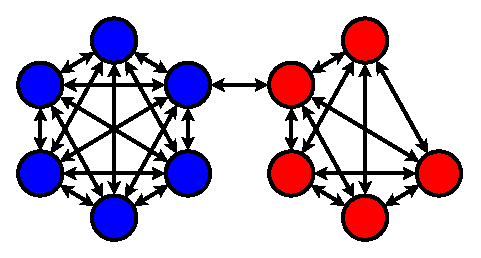
\includegraphics{figures/unl-clique-disjoint.eps}
    \caption{Disjoint UNL}
    \label{fig:unl-clique-disjoint}
\end{figure}

\begin{figure}
    \centering
    
\includegraphics{figures/unl-clique-disjoint-blockchain.eps}
    \caption{Forked blockchain}
    \label{fig:unl-clique-disjoint-blockchain}
\end{figure}

\begin{figure}
    \centering
    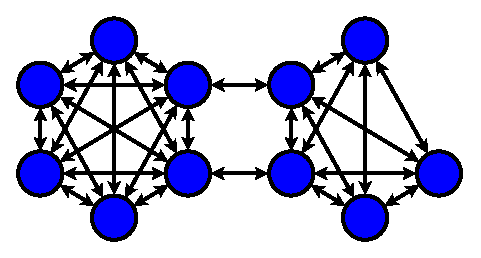
\includegraphics{figures/unl-clique-consensus.eps}
    \caption{UNL cliques in consensus}
    \label{fig:unl-clique-consensus}
\end{figure}

\begin{figure}
    \centering
    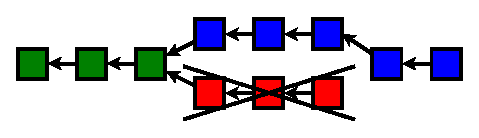
\includegraphics{figures/unl-clique-reorganized-blockchain.eps}
    \caption{Post-fork reorganization}
    \label{fig:unl-clique-post-fork}
\end{figure}


\subsection{Choosing the Unique Node List}
\label{choosing-the-unl}

How should Ripple node administrators pick their Unique Node List? Ripple Labs
provides little, if any, concrete advice beyond the ``starter UNL'' they
provide. Let's look at this problem from another angle: Why shouldn't a node
operator just use the default UNL?

Let's assume the node operator does not know what UNL other nodes in the
economic majority have chosen to use. They do however know the default UNL
provided by Ripple Labs, and they have a reasonable belief that other node
operators also know that UNL and may also be using it. The node operator's goal
is to limit losses; the best case is their node stays in consensus with other
nodes. Second best is they suffer a denial of service attack causing their node
to stop processing some or all transactions. Worst case is their node accepts
transactions that other nodes do not, making possible double-spend attacks.
Table \ref{tbl:unl-outcomes} shows the outcomes of various possible
decisions by them and other node operators, ranging from $100\%$ default UNL,
$50\%$ default UNL, and $10\%$ default UNL.

In every circumstance node operators can reduce the risk of losses due to
consensus failures by removing non-default UNL entries, with the least risky
option being to simply stick with the default UNL of $100\%$ Ripple Labs
controlled nodes. This is particularly acute given the low profit margins of
many financial transactions: while a denial-of-service halts incoming revenue,
a double-spend attack can quickly drain working capital, quite possibly without
any hope of ever recovering the stolen funds.

A closely related issue is what incentive does a node operator have to publicly
perform validation services? Ripple currently has no compensation mechanism for
public validators, yet validation at minimum raises potential legal issues such
as lawsuits for negligence or aiding financial crimes. Again, the least-risk
option is to not publicly validate the Ripple ledger.

\begin{table}
    \centering

    \begin{tabular}{cc|c|c|c}
        \multicolumn{2}{c}{} & \multicolumn{3}{c}{Majority} \\
        \multicolumn{2}{c}{} & $100\%$ & $50\%$ & $10\%$ \\ \cline{3-5}
        \multirow{3}{*}{Local} & $100\%$ & Consensus & DoS & DoS \\ \cline{2-5}
        ~ & $50\%$ & DoS & DoS & Double-spend \\ \cline{2-5}
        ~ & $10\%$ & Double-spend & Double-spend & Double-spend \\
    \end{tabular}

    \caption{Worst-case outcomes of default UNL \% choices}
    \label{tbl:unl-outcomes}
\end{table}


\section{Attack Scenarios}

To evaluate potential attacks on the Ripple network we look at three factors:

\begin{itemize}

    \item \textbf{Type:} What is the effect of the attack? Denial of Service
          and/or theft? Or is the attack mostly useful in preparation for another
          type of attack?

    \item \textbf{Cost:} What is a probable minimum cost to carry out the attack, for
          the people able to do the attack? For instance, a technical attack
          that can be launched by ``bored teenagers'' will have an essentially
          zero cost while a long-term rewrite of a proof-of-work blockchain has
          a reasonably well-defined cost.

    \item \textbf{Scope:} Who is affected by the attack? Is this a targeted attack,
          mainly affecting a one or two targets? An attack with broad impact? Or
          an attack with global impact on all Ripple users?

    \item \textbf{Duration:} How long will it take before the attack is
          neutralized?  This may be a matter of hours to write and distribute a
          simple software patch\footnote{The author personally stopped the
          CVE-2013-4627 attack on the Bitcoin network in a few hours of rushed
          work in the middle of the night.}, to indefinitely long for some
          attacks where recovery is impossible.

    \item \textbf{Probability:} How likely is it for the Ripple network to be
          attacked this way?

\end{itemize}

We do \emph{not} try to determine the monetary impact of the attack, because we
are unable to predict how the Ripple network will be used. For instance, while
a double-spend attack may have the same basic impact on a $\$100/\text{day}$
small business as it would on a $\$1,000,000,000/\text{day}$ multinational, the
latter could lose orders of magnitude more money for what it at a technical
level basically the same attack. A closely issue with attempting to predict
monetary losses is that at some point losses can be sufficiently high that they
create situations where social consensus can decide that the losses simply must
be reversed. For instance, Vericoin community chose to do a hard-fork of their
alt-currency to undo the impact of a major theft.\cite{coindesk-vericoin}


\subsection{Consensus Split}

\begin{center}
    \begin{tabular}{c|c|c|c|c}
        Type & Cost & Scope & Duration & Probability \\ \hline
        DoS   & $\$0$ & Global & Hours & Very High \\
        Theft & $\$1\text{k}$ & Targeted & Hours & Medium
    \end{tabular}
\end{center}

The attacker exploits a difference in behavior between different
implementations/versions of the Ripple protocol. The result of the attack can
be a simple denial of service due to the Ripple network being unable to process
transactions, or with more sophistication, the attacker can fork the Ripple
ledger/blockchain and use the fork to double-spend. The attack is stopped by
identifying it, and then distributing software patches. Provided the Ripple
network is well monitored consensus split attacks can be stopped fairly
quickly; the March 2013 Bitcoin chain fork\cite{bip50} was resolved in a matter
of hours by contacting mining pools. A similar response could happen on Ripple
by contacting validating nodes commonly used in UNLs.\footnote{Another reason
to use the UNL provided Ripple Labs.}

Note that a consensus split may also happen by accident; prior consensus splits
in cryptocurrency systems have almost always been accidental. Equally, that
consensus splits can happen by accident clearly shows that the minimum cost to
perform this attack is zero. However, due to the limited number of consensus
bugs available to exploit in a given (set of) versions of the Ripple protocol
in use and the fast response time possible to consensus splits the potential of
this class of attack for long-term attacks on the network is limited.

Risk factors:

\begin{itemize}

    \item The main implementation of the Ripple protocol, \texttt{rippled}, does
        not cleanly separate the consensus-critical part of the codebase from
        the non-consensus-critical part.\footnote{The consensus-critical
            portions of Bitcoin Core codebase are currently being separated
            into a stand-alone \texttt{libconsensus} library.}

    \item The Ripple protocol itself is extremely complex, with many different
          types of transactions, and all functionality being implemented directly
          in the protocol itself.

    \item Improvements to Ripple frequently require changing the
          consensus-critical codebase rather than user software. For instance
          while on Bitcoin the implementation of multisig was possible without
          modification to the protocol\cite{bip19} in Ripple the lack of
          extension capabilities such as scripting require a consensus-critical
          change.\cite{ripple-wiki-multisign}\footnote{P2SH was \emph{not}
          required for multisig to be implemented.}

\end{itemize}


\subsection{Transaction Flood}

\begin{center}
    \begin{tabular}{c|c|c|c|c}
        Type & Cost & Scope & Duration & Probability \\ \hline
        DoS & $>\$100\text{k}$ & Broad & Varies & Low
    \end{tabular}
\end{center}

The attacker creates large numbers of transactions - either covertly or
overtly - until the Ripple network fails due to overload, or more likely,
Ripple users are priced out of their ability to use the Ripple network.
Transactions pay a minimum fee per transaction by destroying XRP; the fee per
transaction is set by a vote between all validators on the UNL list. In the
short to medium term such an attack would quickly drive up that fee. A
successful attack requires deep pockets as the attacker must out-spend other
Ripple users.


Risk factors:

\begin{itemize}

    \item Ripple Labs plans\cite{cointelegraph-ripple-aml} to require verified
        user identification to use the Ripple network in the near future.  When
        implemented this will make it easy to determine who is doing a covert
        transaction flood attack and restrict their access to the network.

    \item The global consensus ledger has inherently poor $O(n^2)$ scaling;
        even in the absence of a malicious attack the poor scalability of the
        ledger is a threat to the viability of Ripple.

    \item A clever attacker wishing to overtly attack the Ripple network can
        masquerade their traffic as legit economic activity. From the point of
        view of Ripple Labs - a major XRP owner - such an attack may not even
        be considered an attack!\footnote{Similar to the debates in the Bitcoin
        ecosystem about whether or not fee-paying uses of the Bitcoin
        blockchain for non-Bitcoin-denominated transactions constitute
        ``attacks''.}

    \item Attacking the poor scalability of Ripple is highly synergistic with
        attacks depending on the high centralization of the Ripple network as
        even ``unsuccessful'' scalability attacks drive further centralization.
        For instance, if the response to a scalability attack is for Ripple
        Labs to beef up the validation nodes they control, and users stop
        running full nodes themselves, the network is more vulnerable to any
        attacks on those centrally managed validation nodes.

\end{itemize}


\subsection{Coercion of Validators}

\begin{center}
    \begin{tabular}{c|c|c|c|c}
        Type & Cost & Scope & Duration & Probability \\ \hline
        DoS & $>\$100\text{k}$ & Targeted & Indefinite & High \\
        DoS & $>\$1\text{M}$ & Global & Indefinite & Medium \\
        Theft & $>\$100\text{k}$ & Targeted & Indefinite & Medium \\
        Theft & $>\$1\text{M}$ & Global & Indefinite & Low
    \end{tabular}
\end{center}

Validators are coerced through political/legal/criminal means into attacking
some or all Ripple users by preventing valid transactions from entering the
ledger (DoS) and/or by allowing invalid transactions to enter the ledger.
(theft) The cost estimates above are very rough, and assuming the attack is via
legal means; the cost may potentially be as low as zero in some scenarios like
blackmail. In preparation for this attack the attackers may also attempt to
reduce the number of validators by with, for instance, a transaction flood
attack.

Risk factors:

\begin{itemize}

    \item The default UNL list and incentives against operating or using
        non-official validators discussed in Section \ref{choosing-the-unl}
        significantly increase the effectiveness of a coercion attack as nearly
        all Ripple users will be affected. Equally, in the event of a coercion
        attack there are still significant downsides to adopting a different
        UNL.

    \item Similarly this attack is synergistic with transaction flooding and
        other attacks on the scalability of the network, reducing the number of
        validators that need to be coerced.

    \item The \texttt{rippled} node implementation does not check full history. This
        means if validators sign an invalid ledger, the transactions that make
        it invalid can be hidden from Ripple users. Equally, even with
        detection, the fact that Ripple users can be asked to simply
        restart/reinstall their nodes to get past the invalid history may
        significantly reduce the social barriers to creating an invalid ledger.

    \item The Ripple protocol is constructed such that it is possible to create
        many, although not all, types of fraud
        proofs\cite{irc-btcdev-gmaxwell-fraud-proof, btctalk-pkt-fraud-proofs}
        required to prove an invalid ledger. While the software does not
        currently implement fraud proofs, this is functionality that could be
        added in the future without a change to the consensus. If widely used
        fraud proofs could prevent some types of coercion attacks that force
        validators to create invalid ledgers by making it likely for the result
        of the attack to be DoS rather than profitable theft. In short, the
        attack would simply shut the Ripple network down for all users rather
        than result in a successful theft.

    \item Some people would argue that the recently announced
        plans\cite{cointelegraph-ripple-aml} to require verified user
        identification to use the Ripple network in the near future are an
        example of a successful coercion attack. It can be argued that Ripple
        Labs is increasing the risk of coercion attacks by simultaneously
        adopting a ``regulator friendly'' position and promoting the use of
        Ripple across many different jurisdictions.

\end{itemize}

\subsection{Software Backdoor}

\begin{center}
    \begin{tabular}{c|c|c|c|c}
        Type & Cost & Scope & Duration & Probability \\ \hline
        Varies & $\$0$ & Broad & Weeks & High \\
    \end{tabular}
\end{center}

The attacker inserts a backdoor into a widely used Ripple protocol
implementation. (e.g. the \texttt{rippled} node software) The attacker may be an
internal Ripple Labs employee, an external member of the public submitting a
pull-request, or they may compromise the software actually downloaded by
end-users by compromising binary or source code hosting. (e.g. GitHub)

Risk factors:

\begin{itemize}

    \item All relevant software is open source, allowing for third-party
        review. Ripple Labs also has a bug bounty program, which can
        incentivise that review.

    \item Ripple Labs appears to use GitHub - a third party -
        as their master source code repository, with development happening
        through pull-requests on GitHub. While this does place trust in a
        third-party, PGP signing source code during development can mitigate
        this risk. However there appears to be no PGP signatures on any git
        commits, giving Ripple Labs little ability to audit who wrote what
        code.

    \item \textbf{Currently Ripple Labs does not provide a secure way to
        download any of their software.} While binaries are available, the
        mechanism to download them is a Ubuntu package repository over insecure
        HTTP; while source code is available through git, neither commits nor
        release tags are signed in anyway. \textbf{This is a serious omission
        that has lead to significant monetary losses in the past.} Ripple Labs
        should be following industry best-practice by signing git commits and
        tags\cite{wladimir-git-pgp} as well as PGP signing their Ubuntu
        packages.

\end{itemize}


\subsection{Theft of Validator Secret Keys}

\begin{center}
    \begin{tabular}{c|c|c|c|c}
        Type & Cost & Scope & Duration & Probability \\ \hline
        Precursor & $\$0$ & N/A & N/A & Unknown \\
    \end{tabular}
\end{center}

The attacker steals illegitimate control of the secret keys used by validators,
particularly the validators in the default UNL. The theft may happen via an
exploit, backdoor, compromised hosting company, etc. While not useful for the
attacker in of itself, the stolen keys can be used for further attacks such as
DoS or a simulated ledger attack.

A closely related attack is to compromise the Ripple website, and trick people
into downloading a default UNL list consisting of only attacker controlled
nodes.

Risk factors:

\begin{itemize}

    \item Due to the high centralization of UNL validators, a relatively small
        number of validators need to be compromised for a successful attack.

    \item Most validators are running nearly the same, if not the exact same,
        software, making it likely for backdoor/exploit attack to successfully
        exfiltrate the secret keys. Due to the high consensus-critical
        complexity of the Ripple protocol and lack of a consensus library
        alternate validator implementations are currently infeasible, making it
        difficult to change this situation.

    \item The \texttt{rippled} implementation doesn't yet appear to support separating
        the validation/consensus and signing functionality into different
        machines, or even different user accounts. (possibly Ripple Labs has
        internal-use-only improvements)

    \item Details about the operational security practices of the validators on
        the default UNL is unavailable, making it difficult to assess risk.

    \item The Ripple P2P protocol does make it possible to operate validators
        without the nodes themselves accepting public traffic; the signatures
        produced by the validating nodes are distributed via an anonymizing
        flood-fill network. This setup is recommended by Ripple Labs
        documentation and makes remote attacks significantly more difficult.

\end{itemize}


\subsection{Simulated Ledger}

\begin{center}
    \begin{tabular}{c|c|c|c|c}
        Type & Cost & Scope & Duration & Probability \\ \hline
        Theft & $>\$1\text{k}$ & Targeted & Days & N/A
    \end{tabular}
\end{center}

An attacker with the ability to create signatures from nodes on the UNL can
create an entirely simulated ledger in parallel to the ``official'' Ripple
ledger, containing any transaction the attacker wishes. In conjunction with
sybil attacking the target the attacker can then perform double-spend attacks.
Sybil attacks are relatively cheap, requiring just the acquisition of a large
number of IP addresses, e.g. via cloud hosting and/or botnet rental. In some
situations sybil attacks can even have zero cost, such as the internal IT staff
within the target with access to network infrastructure, the target's ISP, or
government actors with MITM capabilities such as the
NSA.\cite{schneier-nsa-mitm}

Risk factors:

\begin{itemize}

    \item Because the Ripple consensus is determined by signatures creating a
        simulated ledger is a zero-cost attack, the ``costless
        simulation''\cite[4.2]{apoelstra-on-stake} problem. Proof-of-work
        ledgers in comparison have very well-defined costs that discourage
        attacks and incentivise detection.\footnote{On the Bitcoin network even
            if the attacker can steal the hashing power needed to simulate
        history for free the miners involved lose money from the attack and
    have strong monetary incentives to detect and stop it.}

    \item There are no direct incentives built into the Ripple protocol to
        discourage validators from allowing their private keys to sign
        simulated ledgers. By comparison the Slasher proof-of-stake algorithm
        attempts to disincentivise simulated history by destroying valuable
        bonds owned up by participants in the consensus
        process.\cite{ethereum-blog-slasher}

    \item The lack of incentive may invite coercion attacks, as the validators
        being coerced into signing a simulated ledger have no direct incentive
        not too. For instance a court could order a validator to assist in a
        simulation attack on a target as a way of recovering funds held by the
        target.

    \item Simulation attacks are made significantly easier by the fact that the
        Ripple consensus protocol will remove validators from the UNL if they
        appear to have failed.\cite[3.4.2]{ripple-consensus-paper} With the
        target sybil attacked the attacker can prevent the target from learning
        that the other validators have \emph{not} failed. When those validators
        are removed from the UNL due to the simulated failure the attacker does
        not need to compromise/coerce as many validators as before. Equally, if
        the target is using network split detection, the attacker can make the
        non-compromised validators \emph{actually} fail as preparation for the
        attack. Again, the lack of incentive to run a validator is problematic.

\end{itemize}


\section{Attack Flowchart}

Figure \ref{fig:attack-flowchart} shows some of the stronger synergies between
different attacks.

Let's go through a full scenario involving multiple attacks at once.  Ripple
Labs has diversified their default UNL such that the $80\%$ of the validators
are run by publicly known institutions evenly spread across the following five
countries, United States, France, Switzerland, Russia, and China, with the
remaining fifth being controlled by pseudoanonymous ``DarkWeb'' entities like
The Silk Road Five, and Agora Market. As any one entity only comprises at most
$1/6\text{th}$ of the UNL no single actor can block transactions.

The Russian government has issued a court order seizing assets of Royal Dutch
Shell, who has recently received funds from Naftogaz Ukraine to develop a new
fracking project. Naftogaz in turn owes Russia for unpaid natural gas imports -
quite a lot more than the funds Shell has, but simply punishing them for
working with Naftogaz is a good start.

By itself Russia is unable to freeze Shell's assets on the Ripple ledger
through coercion of Russian-jurisdiction validators. So Russia begins with a
transaction flood attack, slowly increasing load on the Ripple network to
$10\text{MB}/\text{sec}$ of transactions. As a cover story a new
gambling-oriented MMORPG is created that uses the Ripple ledger to record user
accounts; Ripple Labs is happy to sell them the XRP to cover transaction fees.

The transaction flood results in the pseudoanonymous ``DarkWeb'' validators
quitting - the Tor network is too slow to handle the load, and they worry
they're real identities will be discovered if they move their validator nodes
to clearnet hosting.

At this point Russia's $20\%$ UNL control could simply vote to freeze Shell's
assets, achieving a denial-of-service. However, it's decided it would be better
if the funds were actually recovered instead.

Russia sets up a fake Chinese oil importer, hiring another Chinese company to
do the actual transportation, and has them contact Shell asking to purchase
some oil. They also find a wealthy Chinese investor with \$100 million USD
worth of yuan in an account with a major Chinese bank, and has that investor
``invest'' in the new importer. Meanwhile Russia's cyberwarfare team gets to
work, successfully compromising the Swiss and French validation nodes, and
using the fact that they have agents in major Ukrainian ISPs to sybil attack
the Ukrainian-based Shell office actually handling the sale. They can't
compromise the US nodes - they're on a newer version - but they do happen to
find a new zero-day consensus bug in the newer version.

On the day of the sale unknown to Shell their Ukrainian office's internet
connection is being filtered. The IT staff at their accounting office voices
concern when their Ripple node monitoring tools say that the US validators just
went off-line, although they're somewhat reassured when they hear news that the
US nodes just hit a consensus issue. The captain says there's bad weather
coming in, so they need to leave the port ASAP - with France and Switzerland
approving the transaction they have confidence that the Free World has approved
the money transfer.

What has actually happened is Russian cyberwarfare experts created a fake
consensus using stolen Swiss and French private keys. Russia of course
officially signed this fake consensus, as well as the real consensus, taking
the position this was an above-the-board court ordered operation; China also
signed, but doesn't officially say why. The wealthy Chinese investor
conveniently claims to have suddenly found out about the ``fake'' oil importer
and on the real Ripple ledger has the funds frozen by the Chinese bank backing
them - not a big deal with the money still sitting in the original account he
deposited it too, still under Chinese jurisdiction.

Shell's Ukrainian office finally realises something is wrong after two hours of
debugging, trying to figure out why an exchange wasn't seeing their transaction
attempting to sell that yuan for USD. By that time the ship is in international
waters, and is happy to keep steaming to China, where upon the oil is kept for
the next ten years while the Chinese courts argue what to do with it.

\begin{figure}
    \centering
    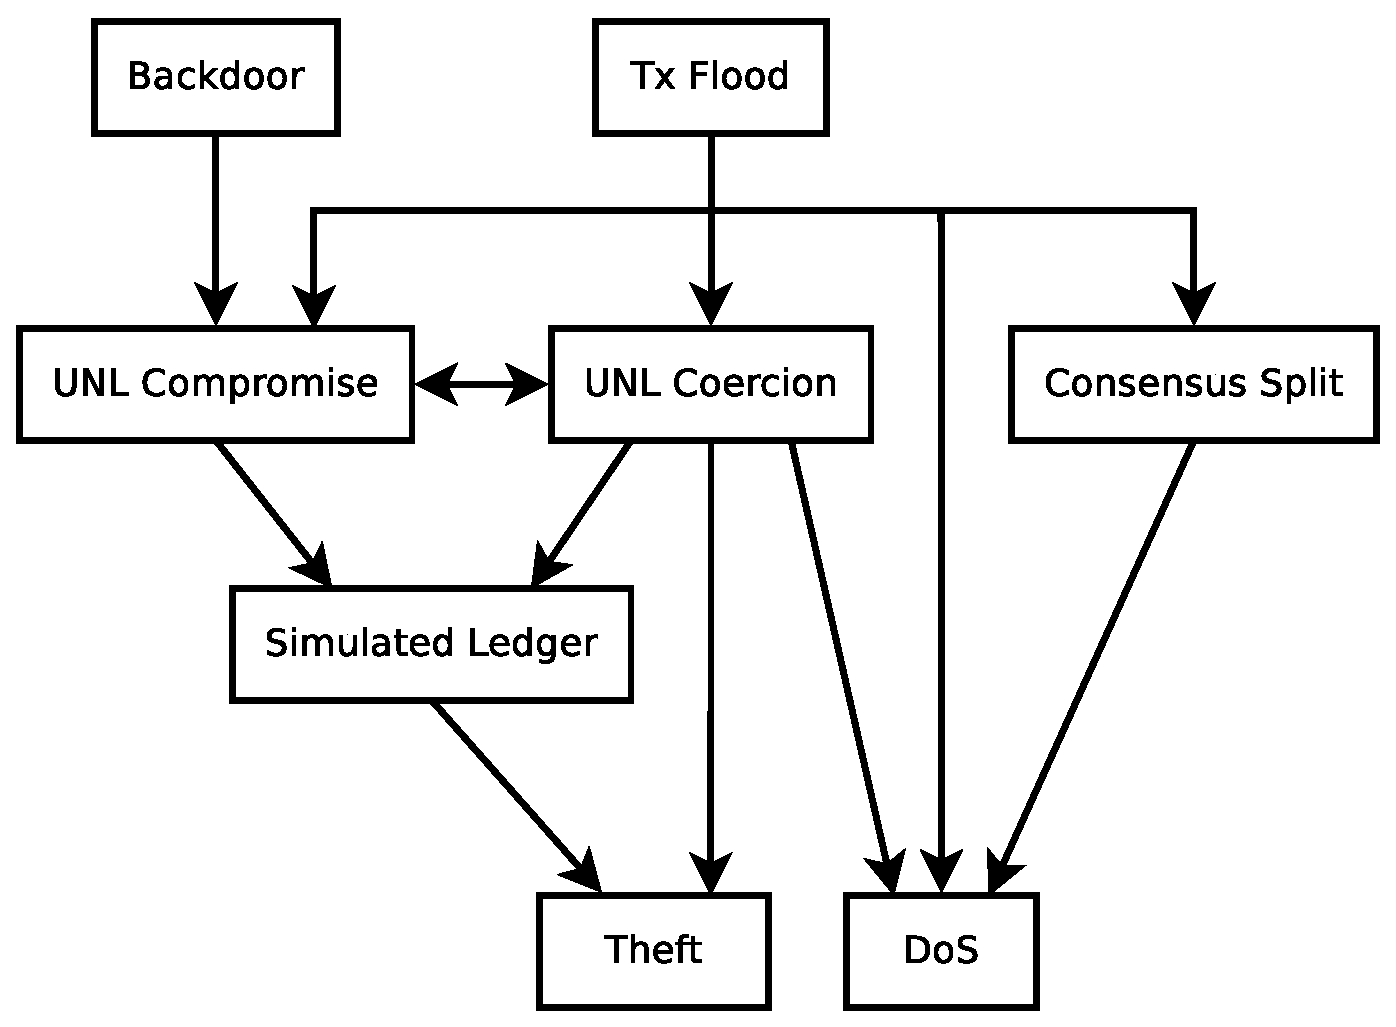
\includegraphics[scale=0.5]{figures/attack-flowchart.eps}
    \caption{Attack flowchart}
    \label{fig:attack-flowchart}
\end{figure}


\section{Conclusions and Future Work}

Nearly all the attack scenarios analysed above are direct outcomes of the need
for consensus; the actual blockchain technology that records the ledger is
relatively uninteresting. That the consensus requirement is for global
consensus rather than the original Ripple's local consensus creates additional
problems such as co-ordination of UNL's, incentives for such co-ordination, and
unclear incentives for validating nodes to validate correctly or honestly.
Finally the requirement of global consensus creates scalability concerns,
privacy concerns, and jurisdictional concerns.

A key question that should be answered in future work is if the goals of the
Ripple system need global consensus at all? If global consensus can be avoided,
or at least its use minimized, many of these issues may go away.

\bibliographystyle{plain}
\bibliography{paper}

\end{document}
